% ===========================================================================
% progress_overall.tex
% Progress presentation for Dagmar & Salah
% Compile: pdflatex -shell-escape progress_overall.tex
% ===========================================================================
\documentclass[10pt,aspectratio=169]{beamer}

% ---- Theme ----------------------------------------------------------------
\usetheme{metropolis}
\usepackage{appendixnumberbeamer}

% Force completely white background
\setbeamercolor{background canvas}{bg=white}
\setbeamercolor{normal text}{fg=black}
\setbeamercolor{alerted text}{fg=ImperialBlue}

% ---- Packages -------------------------------------------------------------
\usepackage[T1]{fontenc}
\usepackage{lmodern}
\usepackage{amsmath,amssymb,amsfonts,mathtools}
\usepackage{bm}
\usepackage{tikz}
\usetikzlibrary{arrows.meta,positioning,fit,shapes.geometric,calc,
                decorations.pathmorphing,decorations.markings,backgrounds,
                shapes.misc,shapes.symbols}
\usepackage{graphicx}
\usepackage{booktabs}
\usepackage{xcolor}
\usepackage{pifont}

% ---- Imperial / Morph Lab palette -----------------------------------------
\definecolor{ImperialBlue}{RGB}{0,62,116}
\definecolor{ImperialLight}{RGB}{0,131,202}
\definecolor{drakeblue}{RGB}{30,90,180}
\definecolor{drakecyan}{RGB}{0,150,180}
\definecolor{drakegreen}{RGB}{40,140,60}
\definecolor{darkred}{RGB}{180,30,30}
\definecolor{expurple}{RGB}{130,40,180}
\definecolor{exolilac}{RGB}{210,180,240}
\definecolor{probecolor}{RGB}{200,60,20}
\definecolor{drakeorange}{RGB}{230,130,30}

\setbeamercolor{frametitle}{bg=ImperialBlue,fg=white}
\setbeamercolor{progress bar}{fg=ImperialLight,bg=ImperialBlue!20}
\setbeamercolor{title separator}{fg=ImperialLight}
\setbeamercolor{block title}{bg=ImperialBlue,fg=white}

% ---- Convenience macros ---------------------------------------------------
\newcommand{\ks}{k_s}
\newcommand{\bc}{b_c}
\newcommand{\kexo}{k_\mathrm{exo}}
\newcommand{\bexo}{b_\mathrm{exo}}
\newcommand{\rexo}{r_\mathrm{exo}}
\newcommand{\tauexo}{\tau_\mathrm{exo}}
\newcommand{\Ke}{K_e}
\newcommand{\Be}{B_e}
\newcommand{\Kehat}{\hat{K}_e}
\newcommand{\Behat}{\hat{B}_e}
\newcommand{\Kp}{K_p}
\newcommand{\Kd}{K_d}
\newcommand{\Kpw}{K_p^\mathrm{weak}}
\newcommand{\Kdw}{K_d^\mathrm{weak}}
\newcommand{\Kpn}{K_p^\mathrm{new}}
\newcommand{\Kdn}{K_d^\mathrm{new}}
\newcommand{\dth}{\Delta\theta}

\newcommand{\checkitem}{\textcolor{drakegreen}{\ding{51}}~}
\newcommand{\crossitem}{\textcolor{darkred}{\ding{55}}~}

% Common tikz styles
\tikzset{
    blk/.style={rectangle, draw=#1, fill=#1!12, thick, rounded corners=2pt,
                minimum height=0.85cm, minimum width=2.0cm, align=center,
                font=\scriptsize\bfseries},
    bigblk/.style={rectangle, draw=#1, fill=#1!10, very thick, rounded corners=3pt,
                   minimum height=1.0cm, minimum width=2.3cm, align=center,
                   font=\small\bfseries},
    arr/.style={-Stealth, thick},
    arrc/.style={-Stealth, thick, #1},
    lbl/.style={font=\tiny, align=center},
}

% ---- Title info -----------------------------------------------------------
\title{Cable-Driven Manipulator + Exosuit}
\subtitle{Progress: Simulation, Control Stack, and Rehab-Inspired Adaptation}
\author{Dipankar Bhattacharya\\\footnotesize{}with Dagmar Sternad \&\ Salah Bazzi}
\institute{Dyson School of Design Engineering~\textbar~Morph Lab, Imperial College London}
\date{\today}

\begin{document}

% ===========================================================================
\maketitle
% ===========================================================================

% ---------------------------------------------------------------------------
\begin{frame}{Outline}
    \tableofcontents
\end{frame}

% ===========================================================================
\section{Simulation Platform}
% ===========================================================================

% ---------------------------------------------------------------------------
\begin{frame}{Two complementary simulators}
\begin{columns}[T,onlytextwidth]
\begin{column}{0.48\textwidth}
\begin{center}
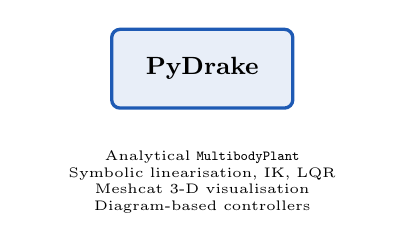
\begin{tikzpicture}[node distance=0.4cm]
    \node[bigblk=drakeblue] (a) {\textbf{PyDrake}};
    \node[lbl, below=of a, text width=4.2cm] {%
        Analytical \texttt{MultibodyPlant}\\
        Symbolic linearisation, IK, LQR\\
        Meshcat 3-D visualisation\\
        Diagram-based controllers};
\end{tikzpicture}
\end{center}
\end{column}
\begin{column}{0.48\textwidth}
\begin{center}
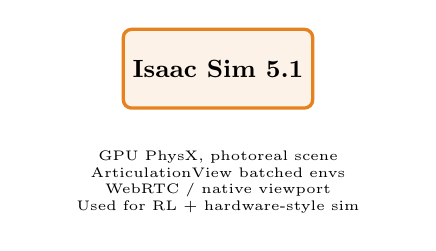
\begin{tikzpicture}[node distance=0.4cm]
    \node[bigblk=drakeorange] (a) {\textbf{Isaac Sim 5.1}};
    \node[lbl, below=of a, text width=4.6cm] {%
        GPU PhysX, photoreal scene\\
        ArticulationView batched envs\\
        WebRTC / native viewport\\
        Used for RL + hardware-style sim};
\end{tikzpicture}
\end{center}
\end{column}
\end{columns}

\vspace{0.4cm}
\begin{center}
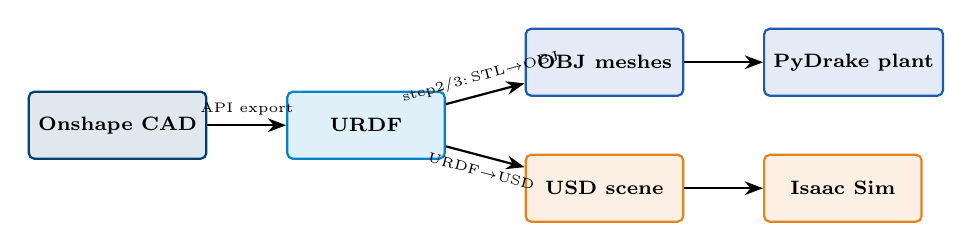
\begin{tikzpicture}[node distance=0.6cm and 1.0cm]
    \node[blk=ImperialBlue] (cad)  {Onshape CAD};
    \node[blk=ImperialLight, right=of cad] (urdf) {URDF};
    \node[blk=drakeblue,     right=of urdf, yshift=0.8cm]  (obj)  {OBJ meshes};
    \node[blk=drakeorange,   right=of urdf, yshift=-0.8cm] (usd)  {USD scene};
    \node[blk=drakeblue,     right=of obj]  (drake) {PyDrake plant};
    \node[blk=drakeorange,   right=of usd]  (isaac) {Isaac Sim};

    \draw[arr] (cad)  -- node[lbl,above]{API export} (urdf);
    \draw[arr] (urdf) -- node[lbl,sloped,above]{step2/3:\,STL$\to$OBJ} (obj);
    \draw[arr] (urdf) -- node[lbl,sloped,below]{URDF$\to$USD} (usd);
    \draw[arr] (obj)  -- (drake);
    \draw[arr] (usd)  -- (isaac);
\end{tikzpicture}
\end{center}

\vfill
{\footnotesize\textit{Single source of truth:} the Onshape assembly drives both pipelines.\\
\texttt{model\_using\_onshape\_to\_robot/manipulator\_cable\_exo\_springs/}}
\end{frame}

% ---------------------------------------------------------------------------
\begin{frame}{From CAD to simulation}
\begin{columns}[T,onlytextwidth]
\begin{column}{0.55\textwidth}
\textbf{Pipeline (scripted):}
\begin{enumerate}
    \item \texttt{step1\_convert\_from\_onshape\_*.sh}\\
          \footnotesize{}Onshape API $\to$ URDF + STL assets
    \item \texttt{step2\_convert\_stl\_to\_obj.py}\\
          \footnotesize{}STL $\to$ OBJ (Drake/Isaac friendly)
    \item \texttt{step3\_urdf\_stl\_to\_obj.py}\\
          \footnotesize{}Rewrite URDF mesh references
    \item \texttt{step4a\_urdf\_fix\_inertia\_for\_exo\_manip.py}\\
          \footnotesize{}Inertia regularisation
\end{enumerate}
\vspace{0.3cm}
\textbf{What we get}
\begin{itemize}
    \item Identical kinematics in both simulators
    \item Pulley + idler frames carried over
    \item Reproducible: rebuild from CAD any time
\end{itemize}
\end{column}
\begin{column}{0.43\textwidth}
\begin{center}
\includegraphics[width=\linewidth]{../pydrake/figures/manipulator.png}\\
{\scriptsize Cable manipulator + exo (Drake render)}
\end{center}
\end{column}
\end{columns}
\end{frame}

% ===========================================================================
\section{System Architecture (Top-Down)}
% ===========================================================================

% ---------------------------------------------------------------------------
\begin{frame}{Three-layer control stack --- the whole picture}
\begin{center}
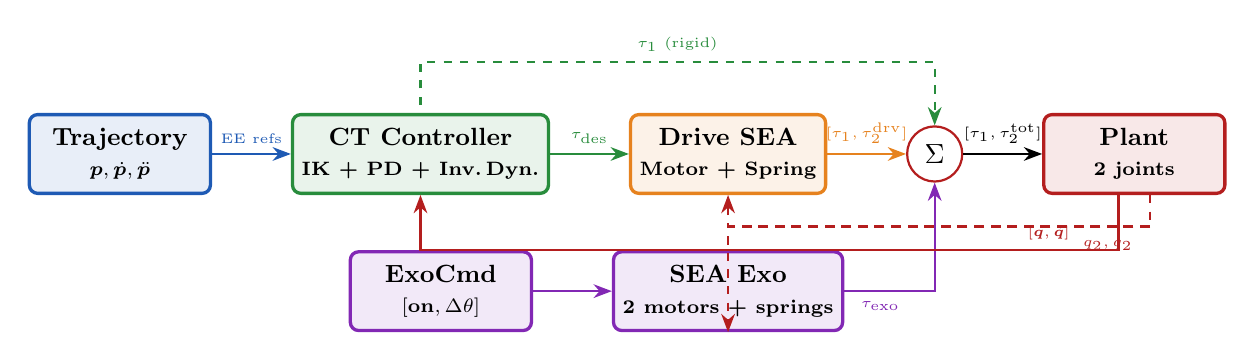
\begin{tikzpicture}[node distance=0.7cm and 1.0cm]
    % Layer blocks
    \node[bigblk=drakeblue]                          (traj)  {Trajectory\\\scriptsize $\bm{p},\dot{\bm{p}},\ddot{\bm{p}}$};
    \node[bigblk=drakegreen, right=of traj]          (ct)    {CT Controller\\\scriptsize IK + PD + Inv.\,Dyn.};
    \node[bigblk=drakeorange, right=of ct]           (sea)   {Drive SEA\\\scriptsize Motor + Spring};
    \node[circle, draw=darkred, thick, right=of sea, minimum size=0.7cm, font=\bfseries] (sum) {$\Sigma$};
    \node[bigblk=darkred,    right=of sum]           (plant) {Plant\\\scriptsize 2 joints};
    \node[bigblk=expurple,   below=of sea]           (exo)   {SEA Exo\\\scriptsize 2 motors + springs};
    \node[bigblk=expurple,   left=of exo]            (ecmd)  {ExoCmd\\\scriptsize $[\text{on},\dth]$};

    % Forward path
    \draw[arrc=drakeblue]   (traj) -- node[lbl,above]{EE refs} (ct);
    \draw[arrc=drakegreen]  (ct)   -- node[lbl,above]{$\tau_\mathrm{des}$} (sea);
    \draw[arrc=drakeorange] (sea)  -- node[lbl,above]{$[\tau_1,\tau_2^\mathrm{drv}]$} (sum);
    \draw[arr]              (sum)  -- node[lbl,above]{$[\tau_1,\tau_2^\mathrm{tot}]$} (plant);
    \draw[arrc=expurple]    (ecmd) -- (exo);
    \draw[arrc=expurple]    (exo.east) -| node[lbl,sloped,below,pos=0.2]{$\tauexo$} (sum.south);

    % Direct rigid line for joint 1
    \draw[arrc=drakegreen, dashed]
        (ct.north) ++(0,0.1) -- ++(0,0.55) -| node[lbl,sloped,above,pos=0.25]{$\tau_1$ (rigid)} (sum.north);

    % Feedback
    \draw[arrc=darkred] (plant.south) ++(-0.2,0) -- ++(0,-0.7) -| node[lbl,sloped,above,pos=0.05]{$[\bm{q},\dot{\bm{q}}]$} (ct.south);
    \draw[arrc=darkred, dashed] (plant.south) ++(0.2,0) -- ++(0,-0.4) -| (sea.south);
    \draw[arrc=darkred, dashed] (plant.south) ++(0.2,0) ++(0,-0.4) -| node[lbl,sloped,below,pos=0.05]{$q_2,\dot{q}_2$} (exo.south);
\end{tikzpicture}
\end{center}

\vspace{-0.2cm}
{\footnotesize
\textbf{Reading the diagram:} the CT controller commands joint torques; joint~2 must pass through a series-elastic cable (Drive SEA) before reaching the plant. The Exo is a second SEA pair acting in parallel on joint~2.}
\end{frame}

% ---------------------------------------------------------------------------
\begin{frame}{Layer 1 --- Computed-Torque controller}
\begin{columns}[T,onlytextwidth]
\begin{column}{0.55\textwidth}
\begin{equation*}
    \boxed{\bm{\tau}_\mathrm{des} = \bm{M}(\bm{q})\,\bm{a}_\mathrm{des} + \bm{h}(\bm{q},\dot{\bm{q}})}
\end{equation*}
\begin{equation*}
    \bm{a}_\mathrm{des} = \Kp(\bm{q}_\mathrm{des} - \bm{q}) - \Kd\,\dot{\bm{q}}
\end{equation*}

\vspace{0.2cm}
\begin{itemize}
    \item $\bm{q}_\mathrm{des}$ from numerical IK on $\bm{p}_\mathrm{ref}(t)$
    \item Feedback linearises rigid-body dynamics
    \item Saturates at motor peak torque
\end{itemize}
\vspace{0.2cm}
\textit{Joint~1 is direct/rigid; only joint~2 has a cable.}
\end{column}
\begin{column}{0.42\textwidth}
\begin{center}
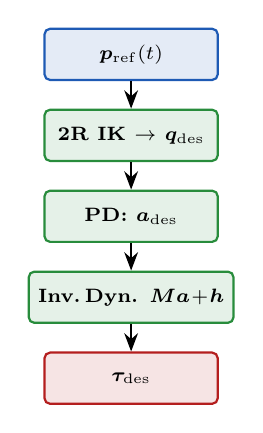
\begin{tikzpicture}[node distance=0.35cm and 0.4cm,
    sblk/.style={rectangle,draw=#1,fill=#1!12,thick,rounded corners=2pt,
                 minimum height=0.65cm,minimum width=2.2cm,
                 align=center,font=\scriptsize\bfseries}]
    \node[sblk=drakeblue]  (p)   {$\bm{p}_\mathrm{ref}(t)$};
    \node[sblk=drakegreen, below=of p]  (ik)  {2R IK $\to$ $\bm{q}_\mathrm{des}$};
    \node[sblk=drakegreen, below=of ik] (pd)  {PD: $\bm{a}_\mathrm{des}$};
    \node[sblk=drakegreen, below=of pd] (id)  {Inv.\,Dyn. $\bm{M}\bm{a}\!+\!\bm{h}$};
    \node[sblk=darkred,    below=of id] (out) {$\bm{\tau}_\mathrm{des}$};

    \draw[arr] (p)  -- (ik);
    \draw[arr] (ik) -- (pd);
    \draw[arr] (pd) -- (id);
    \draw[arr] (id) -- (out);
\end{tikzpicture}
\end{center}
\end{column}
\end{columns}
\end{frame}

% ---------------------------------------------------------------------------
\begin{frame}{Layer 2 --- Drive SEA (joint 2 only)}
\begin{columns}[T,onlytextwidth]
% ---- left: block diagram --------------------------------------------------
\begin{column}{0.50\textwidth}
\begin{center}
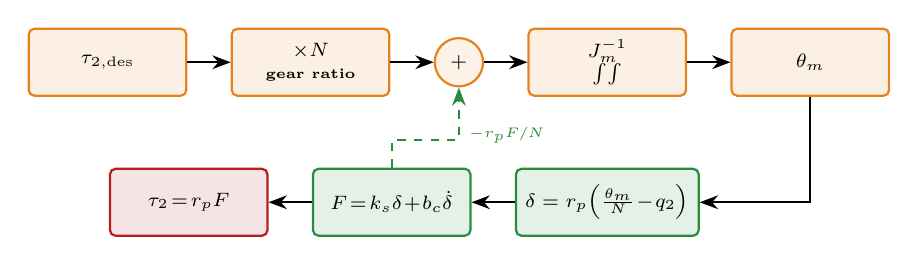
\begin{tikzpicture}[node distance=0.28cm and 0.55cm,
    every node/.style={font=\scriptsize}]
    \node[blk=drakeorange]                          (tau)  {$\tau_{2,\mathrm{des}}$};
    \node[blk=drakeorange, right=of tau]            (gear) {$\times N$\\\tiny gear ratio};
    \node[circle,draw=drakeorange,fill=drakeorange!10,thick,
          minimum size=0.42cm, right=of gear]       (sum1) {$+$};
    \node[blk=drakeorange, right=of sum1]           (mot)  {$J_m^{-1}$\\$\int\!\int$};
    \node[blk=drakeorange, right=of mot]            (theta){$\theta_m$};

    \node[blk=drakegreen, below=0.9cm of mot]       (ext)  {$\delta = r_p\!\left(\tfrac{\theta_m}{N}\!-\!q_2\right)$};
    \node[blk=drakegreen, left=of ext]              (spr)  {$F\!=\!\ks\delta\!+\!\bc\dot\delta$};
    \node[blk=darkred,    left=of spr]              (jt)   {$\tau_2\!=\!r_p F$};

    \draw[arr] (tau)   -- (gear);
    \draw[arr] (gear)  -- (sum1);
    \draw[arr] (sum1)  -- (mot);
    \draw[arr] (mot)   -- (theta);
    \draw[arr] (theta.south) |- (ext.east);
    \draw[arr] (ext)   -- (spr);
    \draw[arr] (spr)   -- (jt);
    % spring force fed back to motor (cable reaction)
    \draw[arr, dashed, drakegreen] (spr.north) -- ++(0,0.35) -|
        (sum1.south) node[pos=0.55,right,font=\tiny,text=drakegreen]{$-r_pF/N$};
\end{tikzpicture}
\end{center}
\end{column}
% ---- right: equations + explanation --------------------------------------
\begin{column}{0.48\textwidth}
\textbf{Key equations}

\medskip
\textbf{1.~Gear ratio} ($\nabla \cdot N$):
\begin{equation*}
    \tau_{m} = N \cdot \tau_{2,\mathrm{des}}
    \quad (\text{torque amplified by }N)
\end{equation*}
The symbol $\nabla\!\cdot\!N$ in block diagrams means \emph{multiply by the gear ratio}; the motor sees $N$ times the joint torque demand, but moves $1/N$ times the joint displacement.

\smallskip
\textbf{2.~Rotor dynamics:}
\begin{equation*}
    J_m\ddot\theta_m = \tau_m - b_m\dot\theta_m - \tfrac{r_p F}{N}
\end{equation*}

\textbf{3.~Spring extension \& force:}
\begin{equation*}
    \delta = r_p\!\left(\tfrac{\theta_m}{N} - q_2\right),\quad
    F = \ks\delta + \bc\dot\delta
\end{equation*}

\textbf{4.~Joint torque:}
\begin{equation*}
    \tau_2 = r_p\,F \quad\text{(cable wraps pulley of radius }r_p\text{)}
\end{equation*}
\end{column}
\end{columns}
\end{frame}

% ---------------------------------------------------------------------------
\begin{frame}{Layer 3 --- Exosuit (Method B: centred elbow pulley)}
\begin{center}
\begin{tikzpicture}[node distance=0.8cm and 1.6cm]
    \node[blk=expurple, minimum width=2.2cm]        (mR)  {Motor R};
    \node[blk=darkred,  below=2.2cm of mR, minimum width=2.2cm]   (mL)  {Motor L};
    
    \node[circle, draw=drakecyan, fill=drakecyan!15, line width=2pt,
          minimum size=1.2cm, right=3.2cm of mR, yshift=-1.1cm]    (pul) {Elbow\\pulley};
    
    \node[blk=drakegreen, right=2.0cm of pul, minimum width=2.2cm] (l2)  {Link 2\\\scriptsize$q_2$};

    \draw[arrc=expurple, line width=1.8pt] (mR.east) -- (pul.north west)
        node[midway,above,font=\scriptsize,text=expurple]{\boldmath$F_R$};
    \draw[arrc=darkred,  line width=1.8pt] (mL.east) -- (pul.south west)
        node[midway,below,font=\scriptsize,text=darkred]{\boldmath$F_L$};
    \draw[arrc=drakeblue,line width=1.2pt] (pul.east) -- (l2.west)
        node[midway,above,font=\scriptsize]{$\boldsymbol{\tau_{\mathrm{exo}}} = r_{\mathrm{exo}}(F_R - F_L)$};
\end{tikzpicture}
\end{center}

\medskip
\begin{columns}[T,onlytextwidth]
\begin{column}{0.48\textwidth}
\textbf{Motor commands} — co-contraction pattern:
\begin{equation*}
\tfrac{\theta_{mR}}{N} = q_{2,\mathrm{des}} + \Delta\theta,\quad
\tfrac{\theta_{mL}}{N} = -q_{2,\mathrm{des}} + \Delta\theta
\end{equation*}
where $\Delta\theta$ \emph{pre-tensions both cables equally}.

\textbf{Cable force} (each, one-sided):
\begin{equation*}
F_i = \max(k_{\mathrm{exo}}\delta_i + b_{\mathrm{exo}}\dot\delta_i,\,0)
\end{equation*}
\end{column}
\begin{column}{0.48\textwidth}
\textbf{Net exosuit torque:}
\begin{equation*}
\tau_{\mathrm{exo}} = r_{\mathrm{exo}}(F_R - F_L)
\end{equation*}

\textbf{Linearised impedance} (around $q_{2,\mathrm{des}}$):
\begin{equation*}
\tau_{\mathrm{exo}} \approx -K_{\mathrm{eff}}\!(q_2-q_{2,\mathrm{des}}) - B_{\mathrm{eff}}\dot{q}_2
\end{equation*}
where $K_{\mathrm{eff}} = 2k_{\mathrm{exo}}r_{\mathrm{exo}}^2$ and $B_{\mathrm{eff}} = 2b_{\mathrm{exo}}r_{\mathrm{exo}}^2$.
\end{column}
\end{columns}
\end{frame}

% ===========================================================================
\section{Behaviour: Transparent vs Activated}
% ===========================================================================

% ---------------------------------------------------------------------------
\begin{frame}{Two operating modes of the exo}
\begin{columns}[T,onlytextwidth]
\begin{column}{0.48\textwidth}
\setbeamercolor{block title}{bg=drakegreen,fg=white}
\begin{block}{Transparent (off)}
\begin{itemize}
    \item Each motor tracks the \emph{actual} $q_2$
    \item Springs stay at rest: $\delta_{R/L}\!=\!0$
    \item $\tauexo \approx 0$ \checkitem the user "doesn't feel" the suit
    \item Baseline tracking performance
\end{itemize}
\end{block}
\end{column}
\begin{column}{0.48\textwidth}
\setbeamercolor{block title}{bg=expurple,fg=white}
\begin{block}{Activated (co-contraction)}
\begin{itemize}
    \item Both cables pre-tensioned: $\dth>0$
    \item Springs deflect with motion
    \item Adds joint stiffness $\Ke$ + damping $\Be$
    \item Resists deviations \emph{about $q_{2,\mathrm{des}}$}
\end{itemize}
\end{block}
\end{column}
\end{columns}

\vspace{0.4cm}
\begin{center}
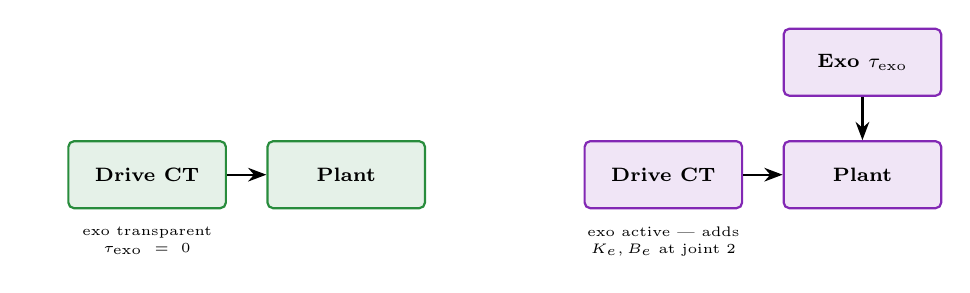
\begin{tikzpicture}[node distance=0.3cm and 0.5cm,
    every node/.style={font=\scriptsize}]
    \node[blk=drakegreen]                        (off1)  {Drive CT};
    \node[blk=drakegreen, right=of off1]         (off2)  {Plant};
    \node[lbl, below=0.1cm of off1, text width=2.8cm]{exo transparent\\$\tauexo\!=\!0$};

    \node[blk=expurple, right=2.0cm of off2]     (on1)  {Drive CT};
    \node[blk=expurple, right=of on1]            (on2)  {Plant};
    \node[blk=expurple, above=0.55cm of on2]     (on3)  {Exo $\tauexo$};
    \node[lbl, below=0.1cm of on1, text width=3.4cm]{exo active --- adds $\Ke,\Be$ at joint 2};

    \draw[arr](off1)--(off2);
    \draw[arr](on1)--(on2);
    \draw[arr](on3.south)--(on2.north);
\end{tikzpicture}
\end{center}
\end{frame}

% ---------------------------------------------------------------------------
\begin{frame}{Disturbance test --- circle trajectory + sinusoidal kick}
\textbf{Scenario.} The EE tracks a circle. At $t=8$\,s a 2\,Hz, 2\,Nm sinusoidal torque is injected on joint~2 for $\sim$\,3 cycles. We compare:
\begin{itemize}
    \item \crossitem\textbf{Exo OFF} (transparent): drive CT must handle everything
    \item \checkitem\textbf{Exo ON} (dist-sync): exo activates exactly during the disturbance
\end{itemize}

\vspace{0.3cm}
\begin{columns}[T,onlytextwidth]
\begin{column}{0.48\textwidth}
\centering\textbf{\textcolor{darkred}{Exo OFF}}\\
\includegraphics[width=\linewidth]{../../../plots/sea_exo_kexo8000_dth0.10_exo_off_20260520_132857_manip.png}
\end{column}
\begin{column}{0.48\textwidth}
\centering\textbf{\textcolor{expurple}{Exo ON (dist-sync)}}\\
\includegraphics[width=\linewidth]{../../../plots/sea_exo_kexo8000_dth0.50_exo_dist_sync_20260520_132422_manip.png}
\end{column}
\end{columns}
\end{frame}

% ---------------------------------------------------------------------------
\begin{frame}{Exo-side diagnostics --- where the help comes from}
\begin{columns}[T,onlytextwidth]
\begin{column}{0.48\textwidth}
\centering\textbf{\textcolor{darkred}{Exo OFF}}\\
\includegraphics[width=\linewidth]{../../../plots/sea_exo_kexo8000_dth0.10_exo_off_20260520_132857_exo.png}
\end{column}
\begin{column}{0.48\textwidth}
\centering\textbf{\textcolor{expurple}{Exo ON (dist-sync)}}\\
\includegraphics[width=\linewidth]{../../../plots/sea_exo_kexo8000_dth0.50_exo_dist_sync_20260520_132422_exo.png}
\end{column}
\end{columns}

\vspace{0.2cm}
\setbeamercolor{block title}{bg=ImperialBlue,fg=white}
\begin{block}{Key observations}
\begin{itemize}\setlength{\itemsep}{2pt}
    \item OFF: cable forces $\approx\!0$, exo torque $\approx\!0$ during the kick; CT error spikes
    \item ON: $F_R$ and $F_L$ alternate; $\tauexo$ pushes opposite to the disturbance (peak $\sim$\,2\,Nm)
    \item Tracking RMS drops from $\sim$\,14\,mm $\rightarrow$ $\sim$\,11\,mm; peak $q_2$ error roughly halved
\end{itemize}
\end{block}
\end{frame}

% ===========================================================================
\section{Rehab-Inspired Parameter Learning}
% ===========================================================================

% ---------------------------------------------------------------------------
\begin{frame}{Why learn the exo impedance?}
\begin{columns}[T,onlytextwidth]
\begin{column}{0.55\textwidth}
\textbf{Clinical analogy}
\begin{itemize}
    \item Patient (= weak CT) tries to move
    \item Exo (= therapist hand) adds stiffness around the desired trajectory
    \item Patient \emph{learns} how much help they were receiving
    \item Therapist gradually withdraws, patient succeeds alone
\end{itemize}
\end{column}
\begin{column}{0.42\textwidth}
\textbf{Engineering picture}
\begin{itemize}
    \item Weak gains $\Kpw,\Kdw$ cannot track alone
    \item Exo provides $\Ke,\Be$ during a probing phase
    \item We identify $\Kehat,\Behat$ from data
    \item Update CT gains, switch the exo \emph{off}
    \item Now CT alone tracks well
\end{itemize}
\end{column}
\end{columns}

\vspace{0.3cm}
\begin{center}\setbeamercolor{block title}{bg=drakegreen,fg=white}
\begin{beamercolorbox}[wd=0.9\textwidth,rounded=true,shadow=true]{block title}
\centering The exo is a \emph{teacher}, not a permanent crutch.
\end{beamercolorbox}
\end{center}
\end{frame}

% ---------------------------------------------------------------------------
\begin{frame}{Three-phase workflow}
\begin{center}
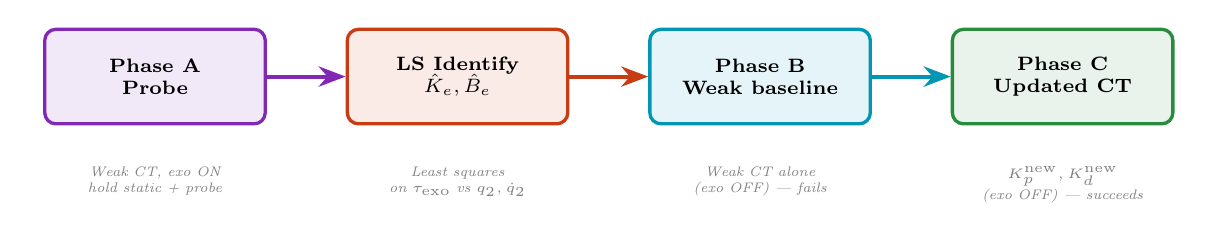
\begin{tikzpicture}[node distance=0.6cm and 1.0cm,
    phase/.style={rectangle, rounded corners=4pt, draw=#1, fill=#1!10, very thick,
                  minimum height=1.2cm, minimum width=2.8cm, align=center,
                  font=\scriptsize\bfseries},
    note/.style={font=\tiny\itshape, text=gray, align=center, text width=3cm},
]
    \node[phase=expurple]                        (A)  {Phase A\\Probe};
    \node[phase=probecolor, right=of A]          (ID) {LS Identify\\$\Kehat,\Behat$};
    \node[phase=drakecyan,  right=of ID]         (B)  {Phase B\\Weak baseline};
    \node[phase=drakegreen, right=of B]          (C)  {Phase C\\Updated CT};

    \draw[arrc=expurple, line width=1.5pt]   (A) -- (ID);
    \draw[arrc=probecolor, line width=1.5pt] (ID) -- (B);
    \draw[arrc=drakecyan, line width=1.5pt]  (B) -- (C);

    \node[note, below=0.4cm of A]  {Weak CT, exo ON\\hold static + probe};
    \node[note, below=0.4cm of ID] {Least squares\\on $\tauexo$ vs $q_2,\dot{q}_2$};
    \node[note, below=0.4cm of B]  {Weak CT alone\\(exo OFF) --- fails};
    \node[note, below=0.4cm of C]  {$\Kpn,\Kdn$\\(exo OFF) --- succeeds};
\end{tikzpicture}
\end{center}

\vspace{0.3cm}
\textbf{Phase A: probe.} Inject $\tau_p(t)=A_p\sin(\omega_p t)$ at joint~2; exo is active with offset $\dth=0.1$ rad. Log $q_2,\dot{q}_2,\tauexo$.

\textbf{Identification.} Stack the regressor
\(\bm{\Phi}=[-(q_2-q_{2,a}),\;-\dot{q}_2]\) and solve
\(\bigl[\Kehat,\Behat\bigr]^\top = (\bm{\Phi}^\top\bm{\Phi})^{-1}\bm{\Phi}^\top\bm{y}\) where $\bm{y}=\tauexo$.

\textbf{Phase C: gain update (additive).}
\[
    \Kpn = \Kpw + \alpha_K\,\Kehat,\qquad
    \Kdn = \Kdw + \alpha_D\,\Behat
\]
\end{frame}

% ---------------------------------------------------------------------------
\begin{frame}{Learning result --- full diagnostic overview}
\begin{center}
\includegraphics[width=0.97\textwidth]{../../../plots/learning_probe_20260520_153204.png}
\end{center}
\end{frame}

% ---------------------------------------------------------------------------
\begin{frame}{Learning result --- panel-by-panel explanation}
\begin{columns}[T,onlytextwidth]
\begin{column}{0.50\textwidth}

\textbf{Phase A — Probing (left column)}
\begin{itemize}\setlength\itemsep{2pt}
    \item \textbf{Top}: $q_2 - q_{2,\mathrm{des}}$ oscillates during the probe window
        (orange shading) as a $1.5\,\mathrm{Hz}$ sine torque is injected.
        The deflection is rich enough for identification.
    \item \textbf{Bar chart}: $\hat{K}_e = 33.4\,\mathrm{Nm/rad}$
        vs.\ ground truth $36.5$ (\textbf{only 8\% error}).
        $\hat{B}_e$ is biased by unmeasured joint friction.
    \item \textbf{Cable forces}: $F_R,F_L$ oscillate in anti-phase
        around the pre-tension baseline, confirming both antagonistic
        cables are active.
    \item \textbf{CT gains updated}: $K_p: 10\to 247$; $K_d: 2\to 4.4$.
        Drive feedback is now strong enough to track without the exo.
    \item \textbf{Tracking error}: updated CT (green) achieves
        RMS $7.3\,\mathrm{mm}$ vs.\ $9.0\,\mathrm{mm}$ weak CT alone (red).
\end{itemize}
\end{column}
\begin{column}{0.48\textwidth}

\textbf{Phase ID --- LS fit (right column)}
\begin{itemize}\setlength\itemsep{2pt}
    \item \textbf{LS fit}: measured $\tau_{\mathrm{exo}}$ (solid) vs.\ fitted
        $-\hat{K}_e(q_2-q_{2,a}) - \hat{B}_e\dot{q}_2$ (dashed).
        Correlation $= 1.000$, RMS residual $= 0.2\,\mathrm{mNm}$ ---
        fit is essentially perfect.
    \item \textbf{Spring extensions}: right cable extends while left
        compresses --- the antagonistic spring behaviour of Method B.
    \item \textbf{Regressor quality}: $-(q_2-q_{2,a})$ and $-\dot{q}_2$
        are phase-shifted sinusoids --- linearly independent, so the LS
        matrix $\bm{\Phi}^\top\bm{\Phi}$ is well-conditioned.
\end{itemize}

\vspace{0.3cm}
\setbeamercolor{block title}{bg=ImperialBlue,fg=white}
\begin{block}{Phase B/C trajectory (bottom right)}
Red = weak CT alone drifts off-circle;
green = updated CT (exo OFF) follows the circle cleanly.
The exo taught the controller enough to succeed on its own.
\end{block}
\end{column}
\end{columns}
\end{frame}

% ===========================================================================
\section{Script 14 Series: Controller Progression}
% ===========================================================================

% ---------------------------------------------------------------------------
\begin{frame}{Scripts 14a–14j: Controller Progression on Cup Manipulator + SEA + Exo}
\vspace{-0.15cm}
{\small
\begin{tabular}{@{}lll@{}}
\toprule
\textbf{Script} & \textbf{Controller} & \textbf{Key Feature} \\
\midrule
14a & Computed Torque (CT) & MATLAB port of PyDrake reference; baseline tracking \\
14b & CCM constant metric ($M{=}P$) & Swaps CT for LQR-Riccati CCM; exo improves $\lambda$ automatically \\
14c & CCM + regional exo & Gaussian mixture of $K_{\mathrm{eff}}$ over joint-space regions \\
14d & CT + RL residual & Scaffold: $\tau{=}\tau_{\text{CT}}+\tau_{\text{RL}}$; 2-layer MLP via REINFORCE \\
14e & CCM SDP, \emph{no exo} & YALMIP block-LMI bisection; finds $\lambda_{\max}$ baseline \\
14f & CCM SDP, \emph{with exo} & Exo adds $-K_{\text{eff}}$ term $\Rightarrow \lambda_{\max}(\text{exo})>\lambda_{\max}(\text{no-exo})$ \\
14g & CCM Slotine formulation & Original SDP (not block-LMI); no-exo vs with-exo side-by-side \\
14h & C3M neural controller & Learned $w_1(x),w_2(x)$ gain matrices; 6D state, exo switched \\
14i & C3M + embedded linear exo & Exo always in $f(x)$; fixes train/deploy mismatch of 14h \\
14j & C3M, 10D augmented state & Adds 4 exo motor states; full certified dual-motor control \\
\bottomrule
\end{tabular}
}
\vspace{0.2cm}
\begin{columns}[T,onlytextwidth]
\begin{column}{0.48\textwidth}
\setbeamercolor{block title}{bg=drakeblue,fg=white}
\begin{block}{Progression logic}
\begin{itemize}
    \item \textbf{14a}: reference baseline (CT)
    \item \textbf{14b–c}: CCM tracking, uniform then regional
    \item \textbf{14d}: RL residual scaffold
    \item \textbf{14e–g}: SDP synthesis \& exo benefit proof
    \item \textbf{14h–j}: learned C3M, increasingly full model
\end{itemize}
\end{block}
\end{column}
\begin{column}{0.48\textwidth}
\setbeamercolor{block title}{bg=drakeorange,fg=white}
\begin{block}{Key takeaways}
\begin{itemize}
    \item Passive exo \emph{provably} increases contraction rate $\lambda$ (14e vs 14f)
    \item CCM $\approx$ CT near origin; advantage grows with disturbance
    \item C3M (14h–j) certifies nonlinear regime the SDP cannot
    \item Embedding exo in $f(x)$ (14i) eliminates train/deploy mismatch
    \item Full 10D state (14j) needed for certified dual-motor exo
\end{itemize}
\end{block}
\end{column}
\end{columns}
\end{frame}

\section{Wrap-up}
% ===========================================================================

% ---------------------------------------------------------------------------
\begin{frame}{Where we are}
\begin{columns}[T,onlytextwidth]
\begin{column}{0.5\textwidth}
\setbeamercolor{block title}{bg=drakegreen,fg=white}
\begin{block}{Done}
\begin{itemize}
    \item Onshape $\to$ URDF $\to$ OBJ \& USD pipeline
    \item CT + Drive SEA + Exo (Method B) in PyDrake
    \item Matching Isaac Sim scene
    \item Disturbance suite: vel/pos/torque/sine/pulse/square
    \item Probe-based identification of $\Ke,\Be$
    \item Additive CT gain update, exo hand-off works in sim
\end{itemize}
\end{block}
\end{column}
\begin{column}{0.48\textwidth}
\setbeamercolor{block title}{bg=drakeorange,fg=white}
\begin{block}{Next}
\begin{itemize}
    \item Bias-free damping identification (separate friction)
    \item Reactive exo activation policy (error-triggered)
    \item Contraction-theory based stability proof
    \item Sim-to-real bridge: motor command logs $\to$ AK60-6 hardware
    \item Subject-study analogue: vary $\dth$, learning rate
\end{itemize}
\end{block}
\end{column}
\end{columns}
\end{frame}

% ---------------------------------------------------------------------------
{\setbeamercolor{background canvas}{bg=ImperialBlue}
\setbeamercolor{normal text}{fg=white}
\begin{frame}[plain]
\begin{center}
\vspace*{2cm}
{\color{white}\Huge\bfseries Thanks!}\\[0.5cm]
{\color{white}\large Happy to dive into any block.}
\end{center}
\end{frame}}

\end{document}
